\documentclass[a4paper]{book}
\usepackage{makeidx}
\usepackage{graphicx}
\usepackage{multicol}
\usepackage{float}
\usepackage{listings}
\usepackage{color}
\usepackage{ifthen}
\usepackage[table]{xcolor}
\usepackage{textcomp}
\usepackage{alltt}
\usepackage{ifpdf}
\ifpdf
\usepackage[pdftex,
            pagebackref=true,
            colorlinks=true,
            linkcolor=blue,
            unicode
           ]{hyperref}
\else
\usepackage[ps2pdf,
            pagebackref=true,
            colorlinks=true,
            linkcolor=blue,
            unicode
           ]{hyperref}
\usepackage{pspicture}
\fi
\usepackage[utf8]{inputenc}
\usepackage[brazil]{babel}
\usepackage{mathptmx}
\usepackage[scaled=.90]{helvet}
\usepackage{courier}
\usepackage{doxygen}
\lstset{language=C++,inputencoding=utf8,basicstyle=\footnotesize,breaklines=true,breakatwhitespace=true,tabsize=8,numbers=left }
\makeindex
\setcounter{tocdepth}{3}
\renewcommand{\footrulewidth}{0.4pt}
\begin{document}
\hypersetup{pageanchor=false}
\begin{titlepage}
\vspace*{7cm}
\begin{center}
{\Large CVMob }\\
\vspace*{1cm}
{\large Gerado por Doxygen 1.7.2}\\
\vspace*{0.5cm}
{\small Sexta, 26 de Novembro de 2010 17:50:15}\\
\end{center}
\end{titlepage}
\clearemptydoublepage
\pagenumbering{roman}
\tableofcontents
\clearemptydoublepage
\pagenumbering{arabic}
\hypersetup{pageanchor=true}
\chapter{Índice dos Componentes}
\section{Hierarquia de Classes}
Esta lista de hierarquias está parcialmente ordenada (ordem alfabética):\begin{DoxyCompactList}
\item \contentsline{section}{AboutDialog}{\pageref{classAboutDialog}}{}
\item \contentsline{section}{Angle}{\pageref{classAngle}}{}
\item \contentsline{section}{model::cvMo}{\pageref{classmodel_1_1cvMo}}{}
\item \contentsline{section}{view::CvMobMainWindow}{\pageref{classview_1_1CvMobMainWindow}}{}
\item \contentsline{section}{cvZoomer}{\pageref{classcvZoomer}}{}
\item \contentsline{section}{controller::FacadeController}{\pageref{classcontroller_1_1FacadeController}}{}
\item \contentsline{section}{FixedPoint}{\pageref{structFixedPoint}}{}
\item \contentsline{section}{model::IExportStrategy}{\pageref{classmodel_1_1IExportStrategy}}{}
\begin{DoxyCompactList}
\item \contentsline{section}{model::ExportText}{\pageref{classmodel_1_1ExportText}}{}
\end{DoxyCompactList}
\item \contentsline{section}{imageViewer}{\pageref{classimageViewer}}{}
\item \contentsline{section}{options}{\pageref{classoptions}}{}
\item \contentsline{section}{model::PhisicsCalc}{\pageref{classmodel_1_1PhisicsCalc}}{}
\item \contentsline{section}{view::Plot}{\pageref{classview_1_1Plot}}{}
\item \contentsline{section}{point}{\pageref{structpoint}}{}
\item \contentsline{section}{model::ProxyOpenCv}{\pageref{classmodel_1_1ProxyOpenCv}}{}
\item \contentsline{section}{reportDialog}{\pageref{classreportDialog}}{}
\end{DoxyCompactList}

\chapter{Índice dos Componentes}
\section{Lista de Componentes}
Aqui estão as classes, estruturas, uniões e interfaces e suas respectivas descrições:\begin{DoxyCompactList}
\item\contentsline{section}{\hyperlink{classAboutDialog}{AboutDialog} }{\pageref{classAboutDialog}}{}
\item\contentsline{section}{\hyperlink{classAngle}{Angle} }{\pageref{classAngle}}{}
\item\contentsline{section}{\hyperlink{classmodel_1_1cvMo}{model::cvMo} }{\pageref{classmodel_1_1cvMo}}{}
\item\contentsline{section}{\hyperlink{classview_1_1CvMobMainWindow}{view::CvMobMainWindow} }{\pageref{classview_1_1CvMobMainWindow}}{}
\item\contentsline{section}{\hyperlink{classcvZoomer}{cvZoomer} }{\pageref{classcvZoomer}}{}
\item\contentsline{section}{\hyperlink{classmodel_1_1ExportText}{model::ExportText} }{\pageref{classmodel_1_1ExportText}}{}
\item\contentsline{section}{\hyperlink{classcontroller_1_1FacadeController}{controller::FacadeController} }{\pageref{classcontroller_1_1FacadeController}}{}
\item\contentsline{section}{\hyperlink{structFixedPoint}{FixedPoint} }{\pageref{structFixedPoint}}{}
\item\contentsline{section}{\hyperlink{classmodel_1_1IExportStrategy}{model::IExportStrategy} }{\pageref{classmodel_1_1IExportStrategy}}{}
\item\contentsline{section}{\hyperlink{classimageViewer}{imageViewer} }{\pageref{classimageViewer}}{}
\item\contentsline{section}{\hyperlink{classoptions}{options} }{\pageref{classoptions}}{}
\item\contentsline{section}{\hyperlink{classmodel_1_1PhisicsCalc}{model::PhisicsCalc} }{\pageref{classmodel_1_1PhisicsCalc}}{}
\item\contentsline{section}{\hyperlink{classview_1_1Plot}{view::Plot} }{\pageref{classview_1_1Plot}}{}
\item\contentsline{section}{\hyperlink{structpoint}{point} }{\pageref{structpoint}}{}
\item\contentsline{section}{\hyperlink{classmodel_1_1ProxyOpenCv}{model::ProxyOpenCv} }{\pageref{classmodel_1_1ProxyOpenCv}}{}
\item\contentsline{section}{\hyperlink{classreportDialog}{reportDialog} }{\pageref{classreportDialog}}{}
\end{DoxyCompactList}

\chapter{Classes}
\hypertarget{classAboutDialog}{
\section{Referência da Classe AboutDialog}
\label{classAboutDialog}\index{AboutDialog@{AboutDialog}}
}
\subsection*{Métodos Públicos}
\begin{DoxyCompactItemize}
\item 
\hypertarget{classAboutDialog_ad96fc2ce8de7568ace543b7c69c71c56}{
{\bfseries AboutDialog} (QWidget $\ast$parent=0)}
\label{classAboutDialog_ad96fc2ce8de7568ace543b7c69c71c56}

\end{DoxyCompactItemize}
\subsection*{Métodos Protegidos}
\begin{DoxyCompactItemize}
\item 
\hypertarget{classAboutDialog_abac18da2759d1b4bb0e5bca856b0efcf}{
void {\bfseries changeEvent} (QEvent $\ast$e)}
\label{classAboutDialog_abac18da2759d1b4bb0e5bca856b0efcf}

\end{DoxyCompactItemize}


A documentação para esta classe foi gerada a partir dos seguintes arquivos:\begin{DoxyCompactItemize}
\item 
/home/luizromario/Romário/Desenvolvimento/C++/CvMob/src/view/aboutdialog.h\item 
/home/luizromario/Romário/Desenvolvimento/C++/CvMob/src/view/aboutdialog.cpp\end{DoxyCompactItemize}

\hypertarget{classAngle}{
\section{Referência da Classe Angle}
\label{classAngle}\index{Angle@{Angle}}
}
\subsection*{Métodos Públicos}
\begin{DoxyCompactItemize}
\item 
\hypertarget{classAngle_a449cc8d99abc3592acad415db189c766}{
void {\bfseries calcValue} (double time)}
\label{classAngle_a449cc8d99abc3592acad415db189c766}

\end{DoxyCompactItemize}
\subsection*{Atributos Públicos}
\begin{DoxyCompactItemize}
\item 
\hypertarget{classAngle_ad1714d4131c99e55870e95899968dcb0}{
int {\bfseries index}}
\label{classAngle_ad1714d4131c99e55870e95899968dcb0}

\item 
\hypertarget{classAngle_a757d6e2314311ce9537f7f0831b1bd4b}{
int {\bfseries color} \mbox{[}3\mbox{]}}
\label{classAngle_a757d6e2314311ce9537f7f0831b1bd4b}

\item 
\hypertarget{classAngle_ad92282b2bbb8a7d1ee9523d7c99fe55c}{
CvPoint2D32f {\bfseries markedPoint}}
\label{classAngle_ad92282b2bbb8a7d1ee9523d7c99fe55c}

\item 
\hypertarget{classAngle_a12101facc34126f3622e99ff2e08bc38}{
QVector$<$ CvPoint2D32f $>$ {\bfseries vertices}}
\label{classAngle_a12101facc34126f3622e99ff2e08bc38}

\item 
\hypertarget{classAngle_ae429845206518a493f61093592c35e19}{
int {\bfseries countVertices}}
\label{classAngle_ae429845206518a493f61093592c35e19}

\item 
\hypertarget{classAngle_a743d8e182082a96727f184fdd761aef4}{
double {\bfseries ang1}}
\label{classAngle_a743d8e182082a96727f184fdd761aef4}

\item 
\hypertarget{classAngle_a5546ad25d88b8e7c83851e03e58e02e8}{
double {\bfseries ang2}}
\label{classAngle_a5546ad25d88b8e7c83851e03e58e02e8}

\item 
\hypertarget{classAngle_ad15e4a83f28b05d3deacf1c4189cd900}{
QVector$<$ double $>$ {\bfseries value}}
\label{classAngle_ad15e4a83f28b05d3deacf1c4189cd900}

\item 
\hypertarget{classAngle_ac46ca515314e708e2122575f0e6a232b}{
QVector$<$ double $>$ {\bfseries velocity}}
\label{classAngle_ac46ca515314e708e2122575f0e6a232b}

\item 
\hypertarget{classAngle_a96b2711867149e4dee85107757bd9cd2}{
QVector$<$ double $>$ {\bfseries time}}
\label{classAngle_a96b2711867149e4dee85107757bd9cd2}

\item 
\hypertarget{classAngle_a3167a68a057586c5c3d92127700032d9}{
QVector$<$ double $>$ {\bfseries acceleration}}
\label{classAngle_a3167a68a057586c5c3d92127700032d9}

\item 
\hypertarget{classAngle_ab06b27256e6503b1c6d3b2dc11694a1e}{
int {\bfseries initFrame}}
\label{classAngle_ab06b27256e6503b1c6d3b2dc11694a1e}

\end{DoxyCompactItemize}


A documentação para esta classe foi gerada a partir dos seguintes arquivos:\begin{DoxyCompactItemize}
\item 
/home/luizromario/Romário/Desenvolvimento/C++/CvMob/src/model/OpenCV/Angle.h\item 
/home/luizromario/Romário/Desenvolvimento/C++/CvMob/src/model/OpenCV/Angle.cpp\end{DoxyCompactItemize}

\hypertarget{classmodel_1_1cvMo}{
\section{Referência da Classe model::cvMo}
\label{classmodel_1_1cvMo}\index{model::cvMo@{model::cvMo}}
}
\subsection*{Métodos Públicos}
\begin{DoxyCompactItemize}
\item 
\hypertarget{classmodel_1_1cvMo_ad880bca0fa96bd7dc51e903771dc878d}{
bool {\bfseries openVideo} (char $\ast$fileName)}
\label{classmodel_1_1cvMo_ad880bca0fa96bd7dc51e903771dc878d}

\item 
\hypertarget{classmodel_1_1cvMo_a1a03ca3bdcac82eca5512c2fe6f72ecf}{
void {\bfseries PutText} (IplImage $\ast$image, char $\ast$text, int x, int y, CvFont $\ast$font, int R, int G, int B)}
\label{classmodel_1_1cvMo_a1a03ca3bdcac82eca5512c2fe6f72ecf}

\item 
\hypertarget{classmodel_1_1cvMo_a4cf4304e1953f7406ce4209dd7083aa5}{
char {\bfseries IsRecording} ()}
\label{classmodel_1_1cvMo_a4cf4304e1953f7406ce4209dd7083aa5}

\item 
\hypertarget{classmodel_1_1cvMo_a6c1a32a5a9375c3113be823fab038f26}{
int {\bfseries Init} ()}
\label{classmodel_1_1cvMo_a6c1a32a5a9375c3113be823fab038f26}

\item 
\hypertarget{classmodel_1_1cvMo_a0725375c5200165de455922900cab149}{
int {\bfseries Init} (char $\ast$file)}
\label{classmodel_1_1cvMo_a0725375c5200165de455922900cab149}

\item 
\hypertarget{classmodel_1_1cvMo_ab3e5215a42261c48f9cc9fc61a6d211c}{
void {\bfseries Record} (FILE $\ast$Frg)}
\label{classmodel_1_1cvMo_ab3e5215a42261c48f9cc9fc61a6d211c}

\item 
\hypertarget{classmodel_1_1cvMo_a870cb535fdfa0eb54c02cf9d3ed3dd3d}{
bool {\bfseries freePoints} ()}
\label{classmodel_1_1cvMo_a870cb535fdfa0eb54c02cf9d3ed3dd3d}

\item 
\hypertarget{classmodel_1_1cvMo_a6ecf231650b5224d623b3845a7a2b0b2}{
bool {\bfseries freeTrajectories} ()}
\label{classmodel_1_1cvMo_a6ecf231650b5224d623b3845a7a2b0b2}

\item 
\hypertarget{classmodel_1_1cvMo_a34ddb95db6a7f92c1a9e2a7f2661db0d}{
void {\bfseries Capture} (int Step)}
\label{classmodel_1_1cvMo_a34ddb95db6a7f92c1a9e2a7f2661db0d}

\item 
\hypertarget{classmodel_1_1cvMo_a8cff44f48900600c7e00e216aecde432}{
void {\bfseries LocatePoints} ()}
\label{classmodel_1_1cvMo_a8cff44f48900600c7e00e216aecde432}

\item 
\hypertarget{classmodel_1_1cvMo_ada4d5e64729342140c0da14fb9ed8b6f}{
void {\bfseries StopRecord} ()}
\label{classmodel_1_1cvMo_ada4d5e64729342140c0da14fb9ed8b6f}

\item 
\hypertarget{classmodel_1_1cvMo_acda84f476a22de805abc0379d5f2956b}{
void {\bfseries SetPlay} (char flag)}
\label{classmodel_1_1cvMo_acda84f476a22de805abc0379d5f2956b}

\item 
\hypertarget{classmodel_1_1cvMo_ab49b9cd2325aa0b89aec73337c3c2eb1}{
void {\bfseries SetStep} (char flag)}
\label{classmodel_1_1cvMo_ab49b9cd2325aa0b89aec73337c3c2eb1}

\item 
\hypertarget{classmodel_1_1cvMo_af8f86598f65d0551bd75deaf764d55c7}{
void {\bfseries DrawGrid} ()}
\label{classmodel_1_1cvMo_af8f86598f65d0551bd75deaf764d55c7}

\item 
\hypertarget{classmodel_1_1cvMo_aded4d096921ed128daa693669a30cfe7}{
void {\bfseries ShowImage} ()}
\label{classmodel_1_1cvMo_aded4d096921ed128daa693669a30cfe7}

\item 
\hypertarget{classmodel_1_1cvMo_ab5a07ca08fa5669b24ff6653319b450c}{
void {\bfseries SetGridStep} (int p)}
\label{classmodel_1_1cvMo_ab5a07ca08fa5669b24ff6653319b450c}

\item 
\hypertarget{classmodel_1_1cvMo_a283696467864bc4902449e82e616dad1}{
void {\bfseries SetGrid} (char onoff)}
\label{classmodel_1_1cvMo_a283696467864bc4902449e82e616dad1}

\item 
\hypertarget{classmodel_1_1cvMo_a2e12fa20bb35668cf56ea0ec3d29453d}{
char {\bfseries IsStepping} ()}
\label{classmodel_1_1cvMo_a2e12fa20bb35668cf56ea0ec3d29453d}

\item 
\hypertarget{classmodel_1_1cvMo_a9499d80fc41ba106aa16226f3cf05853}{
FILE $\ast$ {\bfseries AbreArquivo} (char $\ast$name)}
\label{classmodel_1_1cvMo_a9499d80fc41ba106aa16226f3cf05853}

\item 
\hypertarget{classmodel_1_1cvMo_ac5979160e76b3b63d1ab8fb464561f60}{
int {\bfseries GetNTraject} (int i)}
\label{classmodel_1_1cvMo_ac5979160e76b3b63d1ab8fb464561f60}

\item 
\hypertarget{classmodel_1_1cvMo_afe8eb411031d1df69ea37fdcef7655be}{
int {\bfseries GetPCount} ()}
\label{classmodel_1_1cvMo_afe8eb411031d1df69ea37fdcef7655be}

\item 
\hypertarget{classmodel_1_1cvMo_a75aad254ca3f7f94274df51e11f6a0ae}{
double {\bfseries GetTrajectX} (int \hyperlink{structpoint}{point}, int time)}
\label{classmodel_1_1cvMo_a75aad254ca3f7f94274df51e11f6a0ae}

\item 
\hypertarget{classmodel_1_1cvMo_a310d74ca60e9785fd3ba1fa2a71426a3}{
double {\bfseries GetTrajectY} (int \hyperlink{structpoint}{point}, int time)}
\label{classmodel_1_1cvMo_a310d74ca60e9785fd3ba1fa2a71426a3}

\item 
\hypertarget{classmodel_1_1cvMo_a6c97cef53df42fa1f050bafd154ec099}{
char {\bfseries GetpTipo} (int i)}
\label{classmodel_1_1cvMo_a6c97cef53df42fa1f050bafd154ec099}

\item 
\hypertarget{classmodel_1_1cvMo_a28e2acf82d9be5ed117f8107b56d080c}{
bool {\bfseries ThereIsAngle} ()}
\label{classmodel_1_1cvMo_a28e2acf82d9be5ed117f8107b56d080c}

\item 
\hypertarget{classmodel_1_1cvMo_aabe38046409aa5e9d8e521b5c3c74caa}{
int {\bfseries getTotalFrames} ()}
\label{classmodel_1_1cvMo_aabe38046409aa5e9d8e521b5c3c74caa}

\end{DoxyCompactItemize}
\subsection*{Métodos Públicos Estáticos}
\begin{DoxyCompactItemize}
\item 
static \hyperlink{classmodel_1_1cvMo}{cvMo} $\ast$ \hyperlink{classmodel_1_1cvMo_a2157a33284be205a81f156b4bde126ee}{getInstance} ()
\item 
\hypertarget{classmodel_1_1cvMo_a6d714244c92d2046dd85115045ddcc87}{
static void {\bfseries on\_\-mouseStatic} (int event, int x, int y, int flags, void $\ast$param)}
\label{classmodel_1_1cvMo_a6d714244c92d2046dd85115045ddcc87}

\end{DoxyCompactItemize}
\subsection*{Atributos Públicos}
\begin{DoxyCompactItemize}
\item 
\hypertarget{classmodel_1_1cvMo_ac6f43c674ec1ba3613a5de1fb6fa356d}{
IplImage $\ast$ {\bfseries image}}
\label{classmodel_1_1cvMo_ac6f43c674ec1ba3613a5de1fb6fa356d}

\item 
\hypertarget{classmodel_1_1cvMo_aa61fe0014ce5928ba3e64b82f8cdd718}{
IplImage $\ast$ {\bfseries grey}}
\label{classmodel_1_1cvMo_aa61fe0014ce5928ba3e64b82f8cdd718}

\item 
\hypertarget{classmodel_1_1cvMo_a26242ab4af0785f8d4d580506b719287}{
IplImage $\ast$ {\bfseries prev\_\-grey}}
\label{classmodel_1_1cvMo_a26242ab4af0785f8d4d580506b719287}

\item 
\hypertarget{classmodel_1_1cvMo_a0949ff7d2a407373f79d8903c045c496}{
IplImage $\ast$ {\bfseries pyramid}}
\label{classmodel_1_1cvMo_a0949ff7d2a407373f79d8903c045c496}

\item 
\hypertarget{classmodel_1_1cvMo_aa63a93014a528298d01719d022a8f428}{
IplImage $\ast$ {\bfseries prev\_\-pyramid}}
\label{classmodel_1_1cvMo_aa63a93014a528298d01719d022a8f428}

\item 
\hypertarget{classmodel_1_1cvMo_aeba284894609fbc6e51c674b26a8ae6e}{
IplImage $\ast$ {\bfseries swap\_\-temp}}
\label{classmodel_1_1cvMo_aeba284894609fbc6e51c674b26a8ae6e}

\item 
\hypertarget{classmodel_1_1cvMo_a91c5e8cfb4661f684b91cf4440cae4fd}{
int {\bfseries FilePos}}
\label{classmodel_1_1cvMo_a91c5e8cfb4661f684b91cf4440cae4fd}

\item 
\hypertarget{classmodel_1_1cvMo_a4d01c884181e638cb0f4efb2f5dd7cff}{
int {\bfseries TotFrames}}
\label{classmodel_1_1cvMo_a4d01c884181e638cb0f4efb2f5dd7cff}

\item 
\hypertarget{classmodel_1_1cvMo_ad5c6fe2c1b522b2e3df26c2f685bce37}{
int {\bfseries FrameWidth}}
\label{classmodel_1_1cvMo_ad5c6fe2c1b522b2e3df26c2f685bce37}

\item 
\hypertarget{classmodel_1_1cvMo_a281fc1cb21bcd75417ee5ead9639489a}{
int {\bfseries FrameHeight}}
\label{classmodel_1_1cvMo_a281fc1cb21bcd75417ee5ead9639489a}

\item 
\hypertarget{classmodel_1_1cvMo_afd89ee57cbbf6ad60f109493e44cac81}{
int {\bfseries FrameRate}}
\label{classmodel_1_1cvMo_afd89ee57cbbf6ad60f109493e44cac81}

\item 
\hypertarget{classmodel_1_1cvMo_a579e371d5166ad7acd30bac93ce8a991}{
int {\bfseries Fc}}
\label{classmodel_1_1cvMo_a579e371d5166ad7acd30bac93ce8a991}

\item 
\hypertarget{classmodel_1_1cvMo_a1ca9b4c4e4c1f3cee8523783abee3a36}{
int {\bfseries FcA}}
\label{classmodel_1_1cvMo_a1ca9b4c4e4c1f3cee8523783abee3a36}

\item 
\hypertarget{classmodel_1_1cvMo_a4fd4fcfa22b83888e8e981b8bb469b8d}{
FILE $\ast$ {\bfseries FlRec}}
\label{classmodel_1_1cvMo_a4fd4fcfa22b83888e8e981b8bb469b8d}

\item 
\hypertarget{classmodel_1_1cvMo_ace340726af591b35863919621ad01f2f}{
char {\bfseries FlName} \mbox{[}400\mbox{]}}
\label{classmodel_1_1cvMo_ace340726af591b35863919621ad01f2f}

\item 
\hypertarget{classmodel_1_1cvMo_ae54b11dd4436ae50271b4ced1f406771}{
double {\bfseries Ang} \mbox{[}MAX\_\-TIME\mbox{]}}
\label{classmodel_1_1cvMo_ae54b11dd4436ae50271b4ced1f406771}

\item 
\hypertarget{classmodel_1_1cvMo_a35b6c99c83b452ead06ee7a45ff7d542}{
double {\bfseries TimeA} \mbox{[}MAX\_\-TIME\mbox{]}}
\label{classmodel_1_1cvMo_a35b6c99c83b452ead06ee7a45ff7d542}

\item 
\hypertarget{classmodel_1_1cvMo_a0e1db375957c0fe31b22fcbc6c33fcb6}{
int {\bfseries NApoints}}
\label{classmodel_1_1cvMo_a0e1db375957c0fe31b22fcbc6c33fcb6}

\item 
\hypertarget{classmodel_1_1cvMo_a0ba131797254dd6357db5b5204701eeb}{
char $\ast$ {\bfseries screenName}}
\label{classmodel_1_1cvMo_a0ba131797254dd6357db5b5204701eeb}

\end{DoxyCompactItemize}


\subsection{Métodos}
\hypertarget{classmodel_1_1cvMo_a2157a33284be205a81f156b4bde126ee}{
\index{model::cvMo@{model::cvMo}!getInstance@{getInstance}}
\index{getInstance@{getInstance}!model::cvMo@{model::cvMo}}
\subsubsection[{getInstance}]{\setlength{\rightskip}{0pt plus 5cm}{\bf cvMo} $\ast$ model::cvMo::getInstance (
\begin{DoxyParamCaption}
{}
\end{DoxyParamCaption}
)\hspace{0.3cm}{\ttfamily  \mbox{[}static\mbox{]}}}}
\label{classmodel_1_1cvMo_a2157a33284be205a81f156b4bde126ee}
return the instace. Used to implement Singleton pattern. 

A documentação para esta classe foi gerada a partir dos seguintes arquivos:\begin{DoxyCompactItemize}
\item 
/home/luizromario/Romário/Desenvolvimento/C++/CvMob/src/model/OpenCV/cvMo.h\item 
/home/luizromario/Romário/Desenvolvimento/C++/CvMob/src/model/OpenCV/cvMo.cpp\end{DoxyCompactItemize}

\hypertarget{classview_1_1CvMobMainWindow}{
\section{Referência da Classe view::CvMobMainWindow}
\label{classview_1_1CvMobMainWindow}\index{view::CvMobMainWindow@{view::CvMobMainWindow}}
}
\subsection*{Métodos Públicos}
\begin{DoxyCompactItemize}
\item 
\hypertarget{classview_1_1CvMobMainWindow_ac1c7dd07b0f2fd209b0601f67573636f}{
{\bfseries CvMobMainWindow} (QWidget $\ast$parent=0)}
\label{classview_1_1CvMobMainWindow_ac1c7dd07b0f2fd209b0601f67573636f}

\item 
\hypertarget{classview_1_1CvMobMainWindow_a1d6fd9ebb65b31b6eca0cff126b9eb50}{
void {\bfseries calibratePlots} ()}
\label{classview_1_1CvMobMainWindow_a1d6fd9ebb65b31b6eca0cff126b9eb50}

\end{DoxyCompactItemize}
\subsection*{Métodos Protegidos}
\begin{DoxyCompactItemize}
\item 
\hypertarget{classview_1_1CvMobMainWindow_a58967d72e38ad5355729132bbf18baae}{
void {\bfseries closeEvent} (QCloseEvent $\ast$event)}
\label{classview_1_1CvMobMainWindow_a58967d72e38ad5355729132bbf18baae}

\item 
\hypertarget{classview_1_1CvMobMainWindow_a68ceb75fc638a19a10cf203acd30ca97}{
void {\bfseries keyPressEvent} (QKeyEvent $\ast$e)}
\label{classview_1_1CvMobMainWindow_a68ceb75fc638a19a10cf203acd30ca97}

\end{DoxyCompactItemize}


A documentação para esta classe foi gerada a partir dos seguintes arquivos:\begin{DoxyCompactItemize}
\item 
/home/luizromario/Romário/Desenvolvimento/C++/CvMob/src/view/CvMobMainWindow.h\item 
/home/luizromario/Romário/Desenvolvimento/C++/CvMob/src/view/CvMobMainWindow.cpp\end{DoxyCompactItemize}

\hypertarget{classcvZoomer}{
\section{Referência da Classe cvZoomer}
\label{classcvZoomer}\index{cvZoomer@{cvZoomer}}
}
\subsection*{Métodos Públicos}
\begin{DoxyCompactItemize}
\item 
\hypertarget{classcvZoomer_a2673d92b597dda1d7d0f79ac13928143}{
{\bfseries cvZoomer} (QwtPlotCanvas $\ast$canvas)}
\label{classcvZoomer_a2673d92b597dda1d7d0f79ac13928143}

\item 
\hypertarget{classcvZoomer_a111b7945c477ed74552405acff9e715f}{
virtual QwtText {\bfseries trackerText} (const QwtDoublePoint \&pos) const }
\label{classcvZoomer_a111b7945c477ed74552405acff9e715f}

\end{DoxyCompactItemize}


A documentação para esta classe foi gerada a partir do seguinte arquivo:\begin{DoxyCompactItemize}
\item 
/home/luizromario/Romário/Desenvolvimento/C++/CvMob/src/view/graphs/cvZoomer.h\end{DoxyCompactItemize}

\hypertarget{classmodel_1_1ExportText}{
\section{Referência da Classe model::ExportText}
\label{classmodel_1_1ExportText}\index{model::ExportText@{model::ExportText}}
}
Diagrama de Hierarquia para model::ExportText:\begin{figure}[H]
\begin{center}
\leavevmode
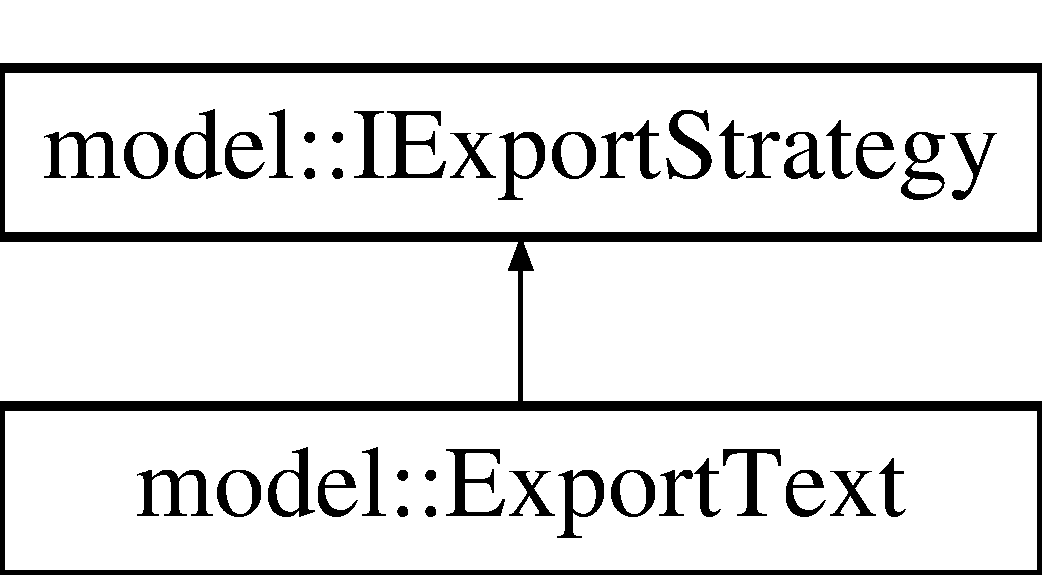
\includegraphics[height=2.000000cm]{classmodel_1_1ExportText}
\end{center}
\end{figure}
\subsection*{Métodos Públicos}
\begin{DoxyCompactItemize}
\item 
\hypertarget{classmodel_1_1ExportText_a69546e170110cd50e751d903b12f6f00}{
void {\bfseries setFile} (char $\ast$filename)}
\label{classmodel_1_1ExportText_a69546e170110cd50e751d903b12f6f00}

\item 
\hypertarget{classmodel_1_1ExportText_a197f589850cb7d3e71a2320be8b2ea17}{
void {\bfseries exportData} (int count, QVector$<$ double $>$ time, QVector$<$ double $>$ velocity, QVector$<$ double $>$ acceleration, QVector$<$ double $>$ work, QVector$<$ CvPoint2D32f $>$ trajectorie, double horizontalRazao, double verticalRazao, int initFrame, QVector$<$ double $>$ velocityX, QVector$<$ double $>$ velocityY, QVector$<$ double $>$ accelerationX, QVector$<$ double $>$ accelerationY)}
\label{classmodel_1_1ExportText_a197f589850cb7d3e71a2320be8b2ea17}

\item 
\hypertarget{classmodel_1_1ExportText_ae882c742d21ac43a2492da884e8b99bc}{
void {\bfseries exportReport} (int count, QVector$<$ double $>$ time, QVector$<$ double $>$ velocity, QVector$<$ double $>$ acceleration, QVector$<$ double $>$ work, QVector$<$ CvPoint2D32f $>$ trajectorie, double horizontalRazao, double verticalRazao, int initFrame, QVector$<$ double $>$ velocityX, QVector$<$ double $>$ velocityY, QVector$<$ double $>$ accelerationX, QVector$<$ double $>$ accelerationY)}
\label{classmodel_1_1ExportText_ae882c742d21ac43a2492da884e8b99bc}

\item 
\hypertarget{classmodel_1_1ExportText_af55398dc07f2e89fea8572f89f027878}{
void {\bfseries closeFile} ()}
\label{classmodel_1_1ExportText_af55398dc07f2e89fea8572f89f027878}

\end{DoxyCompactItemize}


A documentação para esta classe foi gerada a partir dos seguintes arquivos:\begin{DoxyCompactItemize}
\item 
/home/luizromario/Romário/Desenvolvimento/C++/CvMob/src/model/exporter/ExportText.h\item 
/home/luizromario/Romário/Desenvolvimento/C++/CvMob/src/model/exporter/ExportText.cpp\end{DoxyCompactItemize}

\hypertarget{classcontroller_1_1FacadeController}{
\section{Referência da Classe controller::FacadeController}
\label{classcontroller_1_1FacadeController}\index{controller::FacadeController@{controller::FacadeController}}
}
\subsection*{Métodos Públicos}
\begin{DoxyCompactItemize}
\item 
\hypertarget{classcontroller_1_1FacadeController_ae81f0b1634a9ef68fbb494686f41bc47}{
bool {\bfseries openVideo} (char $\ast$fileName)}
\label{classcontroller_1_1FacadeController_ae81f0b1634a9ef68fbb494686f41bc47}

\item 
\hypertarget{classcontroller_1_1FacadeController_a09f651a9faa4911a8c503dea036ec2a0}{
bool {\bfseries openCam} ()}
\label{classcontroller_1_1FacadeController_a09f651a9faa4911a8c503dea036ec2a0}

\item 
\hypertarget{classcontroller_1_1FacadeController_ae55d105dad282a7b6b3eb1ab1c0a029b}{
bool {\bfseries freeFixPoints} ()}
\label{classcontroller_1_1FacadeController_ae55d105dad282a7b6b3eb1ab1c0a029b}

\item 
\hypertarget{classcontroller_1_1FacadeController_a42cf6b38ae4da7a02d3cc431b0285966}{
bool {\bfseries freeTrajPoints} ()}
\label{classcontroller_1_1FacadeController_a42cf6b38ae4da7a02d3cc431b0285966}

\item 
\hypertarget{classcontroller_1_1FacadeController_a90c68e4cb0342788763086db23ac6589}{
bool {\bfseries freeAnglePoints} ()}
\label{classcontroller_1_1FacadeController_a90c68e4cb0342788763086db23ac6589}

\item 
\hypertarget{classcontroller_1_1FacadeController_a36d68b7f0965dc0e83ed8ff8b64d774f}{
void {\bfseries captureFrame} (int frame)}
\label{classcontroller_1_1FacadeController_a36d68b7f0965dc0e83ed8ff8b64d774f}

\item 
\hypertarget{classcontroller_1_1FacadeController_a5cb40e3cbe70514e6d8e7ff8f3040920}{
void {\bfseries calculateData} (int frame)}
\label{classcontroller_1_1FacadeController_a5cb40e3cbe70514e6d8e7ff8f3040920}

\item 
\hypertarget{classcontroller_1_1FacadeController_ad5c8bdbaefbb82adedc25021ac9386f7}{
int {\bfseries getTotalFrames} ()}
\label{classcontroller_1_1FacadeController_ad5c8bdbaefbb82adedc25021ac9386f7}

\item 
\hypertarget{classcontroller_1_1FacadeController_a64c9c514cafb7b60074d6953ddbfc914}{
int {\bfseries getFrameRate} ()}
\label{classcontroller_1_1FacadeController_a64c9c514cafb7b60074d6953ddbfc914}

\item 
\hypertarget{classcontroller_1_1FacadeController_a2e79e6e662fe8738774d367b27bbf2b9}{
double {\bfseries getWinSize} ()}
\label{classcontroller_1_1FacadeController_a2e79e6e662fe8738774d367b27bbf2b9}

\item 
\hypertarget{classcontroller_1_1FacadeController_a96d498f7e679936763230ac3727b7a20}{
void {\bfseries calculateTime} (int actualFrame, char $\ast$buff)}
\label{classcontroller_1_1FacadeController_a96d498f7e679936763230ac3727b7a20}

\item 
\hypertarget{classcontroller_1_1FacadeController_a6c3a420c691056d4f2b14e94b53190aa}{
void {\bfseries setShowVectors} (bool value, char type)}
\label{classcontroller_1_1FacadeController_a6c3a420c691056d4f2b14e94b53190aa}

\item 
\hypertarget{classcontroller_1_1FacadeController_afca92bd1356c4cf313f09f49596b328c}{
void {\bfseries exportTrajectory} (char $\ast$filename)}
\label{classcontroller_1_1FacadeController_afca92bd1356c4cf313f09f49596b328c}

\item 
\hypertarget{classcontroller_1_1FacadeController_a30a3d89c29cb788dba4eb2f5589ba00b}{
void {\bfseries exportReport} ()}
\label{classcontroller_1_1FacadeController_a30a3d89c29cb788dba4eb2f5589ba00b}

\item 
\hypertarget{classcontroller_1_1FacadeController_a6802a6a148259bba9976292d6f601a28}{
void {\bfseries setVideoStreamType} (int type)}
\label{classcontroller_1_1FacadeController_a6802a6a148259bba9976292d6f601a28}

\item 
\hypertarget{classcontroller_1_1FacadeController_a8fb6ba016d4f22696e0265f94ae4d612}{
void {\bfseries setRecording} (bool flag)}
\label{classcontroller_1_1FacadeController_a8fb6ba016d4f22696e0265f94ae4d612}

\item 
\hypertarget{classcontroller_1_1FacadeController_a53e99e3218d60f10ecea65f84ca376b4}{
void {\bfseries startCalibration} (double Distance)}
\label{classcontroller_1_1FacadeController_a53e99e3218d60f10ecea65f84ca376b4}

\item 
\hypertarget{classcontroller_1_1FacadeController_a89ea7c34da8b0ec3395e0f6afe6ec830}{
void {\bfseries addVelocity} ()}
\label{classcontroller_1_1FacadeController_a89ea7c34da8b0ec3395e0f6afe6ec830}

\item 
\hypertarget{classcontroller_1_1FacadeController_ab04b2bc7c3bfa51bbbebb3ec3c156673}{
void {\bfseries removeVelocity} ()}
\label{classcontroller_1_1FacadeController_ab04b2bc7c3bfa51bbbebb3ec3c156673}

\item 
\hypertarget{classcontroller_1_1FacadeController_a0866aedc44238d01ce89d4606ef2c710}{
void {\bfseries addAcceleration} ()}
\label{classcontroller_1_1FacadeController_a0866aedc44238d01ce89d4606ef2c710}

\item 
\hypertarget{classcontroller_1_1FacadeController_a59cf57dc35bdb451c680b7a6a72ef10d}{
void {\bfseries removeAcceleration} ()}
\label{classcontroller_1_1FacadeController_a59cf57dc35bdb451c680b7a6a72ef10d}

\item 
\hypertarget{classcontroller_1_1FacadeController_af615ee47767dc5b7518940495f0ec3e6}{
void {\bfseries addTrabalho} ()}
\label{classcontroller_1_1FacadeController_af615ee47767dc5b7518940495f0ec3e6}

\item 
\hypertarget{classcontroller_1_1FacadeController_a4e45b69e2f39dc2191012d49d8061021}{
void {\bfseries removeTrabalho} ()}
\label{classcontroller_1_1FacadeController_a4e45b69e2f39dc2191012d49d8061021}

\item 
\hypertarget{classcontroller_1_1FacadeController_ad6cbc6f4b65e5d234bfbb9b56f97a2ea}{
void {\bfseries setWinSize} (double value)}
\label{classcontroller_1_1FacadeController_ad6cbc6f4b65e5d234bfbb9b56f97a2ea}

\end{DoxyCompactItemize}
\subsection*{Métodos Públicos Estáticos}
\begin{DoxyCompactItemize}
\item 
static \hyperlink{classcontroller_1_1FacadeController}{FacadeController} $\ast$ \hyperlink{classcontroller_1_1FacadeController_a08417d90d1b3acf44ec4b65f0e28aae4}{getInstance} ()
\end{DoxyCompactItemize}


\subsection{Métodos}
\hypertarget{classcontroller_1_1FacadeController_a08417d90d1b3acf44ec4b65f0e28aae4}{
\index{controller::FacadeController@{controller::FacadeController}!getInstance@{getInstance}}
\index{getInstance@{getInstance}!controller::FacadeController@{controller::FacadeController}}
\subsubsection[{getInstance}]{\setlength{\rightskip}{0pt plus 5cm}{\bf FacadeController} $\ast$ controller::FacadeController::getInstance (
\begin{DoxyParamCaption}
{}
\end{DoxyParamCaption}
)\hspace{0.3cm}{\ttfamily  \mbox{[}static\mbox{]}}}}
\label{classcontroller_1_1FacadeController_a08417d90d1b3acf44ec4b65f0e28aae4}
return the instace. Used to implement Singleton pattern. 

A documentação para esta classe foi gerada a partir dos seguintes arquivos:\begin{DoxyCompactItemize}
\item 
/home/luizromario/Romário/Desenvolvimento/C++/CvMob/src/controller/FacadeController.h\item 
/home/luizromario/Romário/Desenvolvimento/C++/CvMob/src/controller/FacadeController.cpp\end{DoxyCompactItemize}

\hypertarget{structFixedPoint}{
\section{Referência da Estrutura FixedPoint}
\label{structFixedPoint}\index{FixedPoint@{FixedPoint}}
}
\subsection*{Atributos Públicos}
\begin{DoxyCompactItemize}
\item 
\hypertarget{structFixedPoint_abbd6af5f960ed2f5073eeeb8d83448bd}{
int {\bfseries index}}
\label{structFixedPoint_abbd6af5f960ed2f5073eeeb8d83448bd}

\item 
\hypertarget{structFixedPoint_a6927c9ffc2d24c8e6dbe50d1eca2ce08}{
int {\bfseries color} \mbox{[}3\mbox{]}}
\label{structFixedPoint_a6927c9ffc2d24c8e6dbe50d1eca2ce08}

\item 
\hypertarget{structFixedPoint_aa6e07a88022b05e9b858b8cbad568572}{
CvPoint2D32f {\bfseries markedPoint}}
\label{structFixedPoint_aa6e07a88022b05e9b858b8cbad568572}

\item 
\hypertarget{structFixedPoint_a2bb8cbec79a11a4207103a27482398c4}{
CvPoint2D32f {\bfseries features} \mbox{[}1\mbox{]}}
\label{structFixedPoint_a2bb8cbec79a11a4207103a27482398c4}

\item 
\hypertarget{structFixedPoint_a831181b3b13bf5e7bc5559264e4c32cf}{
CvPoint2D32f {\bfseries prev\_\-features} \mbox{[}1\mbox{]}}
\label{structFixedPoint_a831181b3b13bf5e7bc5559264e4c32cf}

\item 
\hypertarget{structFixedPoint_aea1b62caa947e534319237e98bd56ee8}{
int {\bfseries initFrame}}
\label{structFixedPoint_aea1b62caa947e534319237e98bd56ee8}

\end{DoxyCompactItemize}


A documentação para esta estrutura foi gerada a partir do seguinte arquivo:\begin{DoxyCompactItemize}
\item 
/home/luizromario/Romário/Desenvolvimento/C++/CvMob/src/model/OpenCV/Point.h\end{DoxyCompactItemize}

\hypertarget{classmodel_1_1IExportStrategy}{
\section{Referência da Classe model::IExportStrategy}
\label{classmodel_1_1IExportStrategy}\index{model::IExportStrategy@{model::IExportStrategy}}
}
Diagrama de Hierarquia para model::IExportStrategy:\begin{figure}[H]
\begin{center}
\leavevmode
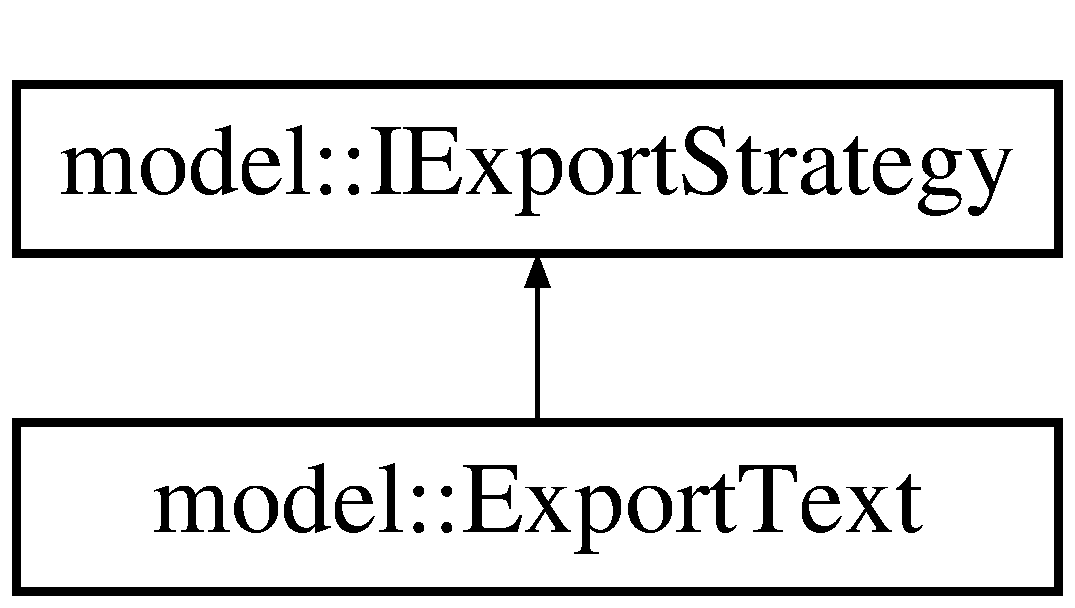
\includegraphics[height=2.000000cm]{classmodel_1_1IExportStrategy}
\end{center}
\end{figure}
\subsection*{Métodos Públicos}
\begin{DoxyCompactItemize}
\item 
\hypertarget{classmodel_1_1IExportStrategy_aecac2597bc3e87a751ead9ac14ad52a1}{
virtual void {\bfseries setFile} (char $\ast$filename)}
\label{classmodel_1_1IExportStrategy_aecac2597bc3e87a751ead9ac14ad52a1}

\item 
\hypertarget{classmodel_1_1IExportStrategy_abf9201b5c3c376fcf14c14658d744329}{
virtual void {\bfseries exportData} (int count, QVector$<$ double $>$ time, QVector$<$ double $>$ velocity, QVector$<$ double $>$ acceleration, QVector$<$ double $>$ work, QVector$<$ CvPoint2D32f $>$ trajectorie, double horizontalRazao, double verticalRazao, int initFrame, QVector$<$ double $>$ velocityX, QVector$<$ double $>$ velocityY, QVector$<$ double $>$ accelerationX, QVector$<$ double $>$ accelerationY)}
\label{classmodel_1_1IExportStrategy_abf9201b5c3c376fcf14c14658d744329}

\item 
\hypertarget{classmodel_1_1IExportStrategy_a829d6500059dc9128a1d084781009dd0}{
virtual void {\bfseries exportReport} (int count, QVector$<$ double $>$ time, QVector$<$ double $>$ velocity, QVector$<$ double $>$ acceleration, QVector$<$ double $>$ work, QVector$<$ CvPoint2D32f $>$ trajectorie, double horizontalRazao, double verticalRazao, int initFrame, QVector$<$ double $>$ velocityX, QVector$<$ double $>$ velocityY, QVector$<$ double $>$ accelerationX, QVector$<$ double $>$ accelerationY)}
\label{classmodel_1_1IExportStrategy_a829d6500059dc9128a1d084781009dd0}

\item 
\hypertarget{classmodel_1_1IExportStrategy_a6197dfc572bc707ecdfe9932a61e73b6}{
virtual void {\bfseries closeFile} ()}
\label{classmodel_1_1IExportStrategy_a6197dfc572bc707ecdfe9932a61e73b6}

\end{DoxyCompactItemize}


A documentação para esta classe foi gerada a partir dos seguintes arquivos:\begin{DoxyCompactItemize}
\item 
/home/luizromario/Romário/Desenvolvimento/C++/CvMob/src/model/exporter/IExportStrategy.h\item 
/home/luizromario/Romário/Desenvolvimento/C++/CvMob/src/model/exporter/IExportStrategy.cpp\end{DoxyCompactItemize}

\hypertarget{classimageViewer}{
\section{Referência da Classe imageViewer}
\label{classimageViewer}\index{imageViewer@{imageViewer}}
}
\subsection*{Sinais}
\begin{DoxyCompactItemize}
\item 
\hypertarget{classimageViewer_a4d18871fbab4e167aa2decf942f5fe1b}{
void {\bfseries updateKeyboard} (int c)}
\label{classimageViewer_a4d18871fbab4e167aa2decf942f5fe1b}

\item 
\hypertarget{classimageViewer_a79add8ded5d97387e9da78e3dc72c9d1}{
void {\bfseries updatWinSize} (double value)}
\label{classimageViewer_a79add8ded5d97387e9da78e3dc72c9d1}

\item 
\hypertarget{classimageViewer_a1ba8b978b417ded69fd5bb4dc9a0734e}{
void {\bfseries closedImgView} ()}
\label{classimageViewer_a1ba8b978b417ded69fd5bb4dc9a0734e}

\end{DoxyCompactItemize}
\subsection*{Métodos Públicos}
\begin{DoxyCompactItemize}
\item 
\hypertarget{classimageViewer_ac8c00c9f17e368cad344aca2ef311d2f}{
void {\bfseries drawImage} (Mat image)}
\label{classimageViewer_ac8c00c9f17e368cad344aca2ef311d2f}

\item 
\hypertarget{classimageViewer_ad0e61a4f5b4beb457964401ef5ad12a0}{
void {\bfseries setImage} (Mat image)}
\label{classimageViewer_ad0e61a4f5b4beb457964401ef5ad12a0}

\end{DoxyCompactItemize}
\subsection*{Atributos Públicos}
\begin{DoxyCompactItemize}
\item 
\hypertarget{classimageViewer_a77b1d347d6909afe154ce307f88d1925}{
QGridLayout {\bfseries imageLayout}}
\label{classimageViewer_a77b1d347d6909afe154ce307f88d1925}

\item 
\hypertarget{classimageViewer_af575ccfa720ae7217af02269aeec72cb}{
QLabel {\bfseries imageLabel}}
\label{classimageViewer_af575ccfa720ae7217af02269aeec72cb}

\item 
\hypertarget{classimageViewer_a42128e897301e2abc44aa53696337c29}{
\hyperlink{classoptions}{options} {\bfseries op}}
\label{classimageViewer_a42128e897301e2abc44aa53696337c29}

\end{DoxyCompactItemize}
\subsection*{Métodos Protegidos}
\begin{DoxyCompactItemize}
\item 
\hypertarget{classimageViewer_ae192d62e031013eb33565dc0cf4e0c48}{
void {\bfseries mousePressEvent} (QMouseEvent $\ast$event)}
\label{classimageViewer_ae192d62e031013eb33565dc0cf4e0c48}

\item 
\hypertarget{classimageViewer_a751e6a74b4a3b537e22d7ec1b21b5e08}{
void {\bfseries mouseMoveEvent} (QMouseEvent $\ast$event)}
\label{classimageViewer_a751e6a74b4a3b537e22d7ec1b21b5e08}

\item 
\hypertarget{classimageViewer_a8791119b74e7d7933406c4793ee01e6a}{
void {\bfseries keyPressEvent} (QKeyEvent $\ast$e)}
\label{classimageViewer_a8791119b74e7d7933406c4793ee01e6a}

\item 
\hypertarget{classimageViewer_aa1ae43c486ad1d68c508ca8d10d52018}{
void {\bfseries closeEvent} (QCloseEvent $\ast$event)}
\label{classimageViewer_aa1ae43c486ad1d68c508ca8d10d52018}

\item 
\hypertarget{classimageViewer_acbc39588ff386cbfc8962d3a2a57b5d4}{
void {\bfseries paintEvent} (QPaintEvent $\ast$event)}
\label{classimageViewer_acbc39588ff386cbfc8962d3a2a57b5d4}

\item 
\hypertarget{classimageViewer_a02b850eb75c7be90df19fcf4d3031039}{
void {\bfseries wheelEvent} (QWheelEvent $\ast$event)}
\label{classimageViewer_a02b850eb75c7be90df19fcf4d3031039}

\end{DoxyCompactItemize}


A documentação para esta classe foi gerada a partir dos seguintes arquivos:\begin{DoxyCompactItemize}
\item 
/home/luizromario/Romário/Desenvolvimento/C++/CvMob/src/view/imageviewer.h\item 
/home/luizromario/Romário/Desenvolvimento/C++/CvMob/src/view/imageviewer.cpp\end{DoxyCompactItemize}

\hypertarget{classoptions}{
\section{Referência da Classe options}
\label{classoptions}\index{options@{options}}
}
\subsection*{Atributos Públicos}
\begin{DoxyCompactItemize}
\item 
\hypertarget{classoptions_a98fde01a409664ff03269abd8e29d6ac}{
int {\bfseries prec}}
\label{classoptions_a98fde01a409664ff03269abd8e29d6ac}

\end{DoxyCompactItemize}


A documentação para esta classe foi gerada a partir dos seguintes arquivos:\begin{DoxyCompactItemize}
\item 
/home/luizromario/Romário/Desenvolvimento/C++/CvMob/src/view/options.h\item 
/home/luizromario/Romário/Desenvolvimento/C++/CvMob/src/view/options.cpp\end{DoxyCompactItemize}

\hypertarget{classmodel_1_1PhisicsCalc}{
\section{Referência da Classe model::PhisicsCalc}
\label{classmodel_1_1PhisicsCalc}\index{model::PhisicsCalc@{model::PhisicsCalc}}
}
\subsection*{Métodos Públicos}
\begin{DoxyCompactItemize}
\item 
double \hyperlink{classmodel_1_1PhisicsCalc_ae2f7e7ac8293bf12c472150d7de8247d}{calculateAxisVelocity} (double S1, double S2, double time)
\item 
double \hyperlink{classmodel_1_1PhisicsCalc_a63df0334920bcc2f8f9313acc2f028fd}{calculateAxisAcceleration} (double S1, double S2, double S3, double S4, double time)
\item 
\hypertarget{classmodel_1_1PhisicsCalc_ac336b208d6ff076b1b7faaf40f841cd8}{
double {\bfseries calculateVelocity} (double Vx, double Vy)}
\label{classmodel_1_1PhisicsCalc_ac336b208d6ff076b1b7faaf40f841cd8}

\item 
\hypertarget{classmodel_1_1PhisicsCalc_a2a3a56dc3e586fce9f85a0424fd7ae4a}{
double {\bfseries calculateAcceleration} (double Ax, double Ay)}
\label{classmodel_1_1PhisicsCalc_a2a3a56dc3e586fce9f85a0424fd7ae4a}

\item 
\hypertarget{classmodel_1_1PhisicsCalc_a7859f3cd01d28d7f64ec67f60dc7cad0}{
double {\bfseries calculateWork} (double dx, double dy, double acceleration)}
\label{classmodel_1_1PhisicsCalc_a7859f3cd01d28d7f64ec67f60dc7cad0}

\end{DoxyCompactItemize}


\subsection{Métodos}
\hypertarget{classmodel_1_1PhisicsCalc_a63df0334920bcc2f8f9313acc2f028fd}{
\index{model::PhisicsCalc@{model::PhisicsCalc}!calculateAxisAcceleration@{calculateAxisAcceleration}}
\index{calculateAxisAcceleration@{calculateAxisAcceleration}!model::PhisicsCalc@{model::PhisicsCalc}}
\subsubsection[{calculateAxisAcceleration}]{\setlength{\rightskip}{0pt plus 5cm}double model::PhisicsCalc::calculateAxisAcceleration (
\begin{DoxyParamCaption}
\item[{double}]{ S1, }
\item[{double}]{ S2, }
\item[{double}]{ S3, }
\item[{double}]{ S4, }
\item[{double}]{ time}
\end{DoxyParamCaption}
)}}
\label{classmodel_1_1PhisicsCalc_a63df0334920bcc2f8f9313acc2f028fd}
usa quatro varia��es de espa�o em um eixo para calcular a acelera��o no eixo. S1= varia��o do frame at� o frame +1 S2= varia��o do frame+1 at� o frame+2 S3= varia��o do frame -\/2 at� o frame -\/1 S4= varia��o do frame-\/1 at� o frame TODO: COLOCAR PARENTESES NO 4$\ast$... \hypertarget{classmodel_1_1PhisicsCalc_ae2f7e7ac8293bf12c472150d7de8247d}{
\index{model::PhisicsCalc@{model::PhisicsCalc}!calculateAxisVelocity@{calculateAxisVelocity}}
\index{calculateAxisVelocity@{calculateAxisVelocity}!model::PhisicsCalc@{model::PhisicsCalc}}
\subsubsection[{calculateAxisVelocity}]{\setlength{\rightskip}{0pt plus 5cm}double model::PhisicsCalc::calculateAxisVelocity (
\begin{DoxyParamCaption}
\item[{double}]{ S1, }
\item[{double}]{ S2, }
\item[{double}]{ time}
\end{DoxyParamCaption}
)}}
\label{classmodel_1_1PhisicsCalc_ae2f7e7ac8293bf12c472150d7de8247d}
usa duas varia��es de espa�o em um eixo para calcular a velocidade no eixo. S1 = varia��o do frame -\/1 at� o frame S2 = varia��o do frame at� o frame +1 

A documentação para esta classe foi gerada a partir dos seguintes arquivos:\begin{DoxyCompactItemize}
\item 
/home/luizromario/Romário/Desenvolvimento/C++/CvMob/src/model/PhisicsCalc.h\item 
/home/luizromario/Romário/Desenvolvimento/C++/CvMob/src/model/PhisicsCalc.cpp\end{DoxyCompactItemize}

\hypertarget{classview_1_1Plot}{
\section{Referência da Classe view::Plot}
\label{classview_1_1Plot}\index{view::Plot@{view::Plot}}
}
\subsection*{Métodos Públicos}
\begin{DoxyCompactItemize}
\item 
\hyperlink{classview_1_1Plot_acc8c8f155ef193c507c5d395883940a6}{Plot} (QString Title, QString AxisXTitle, QString AxisYTitle)
\item 
\hypertarget{classview_1_1Plot_a57aed6ec73a6a51df5e3375662a616bd}{
void {\bfseries addCurve} (int index, int r, int g, int b)}
\label{classview_1_1Plot_a57aed6ec73a6a51df5e3375662a616bd}

\item 
\hypertarget{classview_1_1Plot_a40012744078b511d8bc68579874f557b}{
void {\bfseries setData} (int curve, double $\ast$xData, double $\ast$yData, int sizeData)}
\label{classview_1_1Plot_a40012744078b511d8bc68579874f557b}

\item 
\hypertarget{classview_1_1Plot_abc55871870da2bf0ecff82337b39e883}{
void {\bfseries releaseCurves} ()}
\label{classview_1_1Plot_abc55871870da2bf0ecff82337b39e883}

\item 
\hypertarget{classview_1_1Plot_a3deb3231a1310cfcc4a019ca0952381a}{
void {\bfseries setXAxisTitle} (QString title)}
\label{classview_1_1Plot_a3deb3231a1310cfcc4a019ca0952381a}

\item 
\hypertarget{classview_1_1Plot_a342f6af2316869a294dab1e600764ebc}{
void {\bfseries setYAxisTitle} (QString title)}
\label{classview_1_1Plot_a342f6af2316869a294dab1e600764ebc}

\end{DoxyCompactItemize}


\subsection{Construtores \& Destrutores}
\hypertarget{classview_1_1Plot_acc8c8f155ef193c507c5d395883940a6}{
\index{view::Plot@{view::Plot}!Plot@{Plot}}
\index{Plot@{Plot}!view::Plot@{view::Plot}}
\subsubsection[{Plot}]{\setlength{\rightskip}{0pt plus 5cm}view::Plot::Plot (
\begin{DoxyParamCaption}
\item[{QString}]{ Title, }
\item[{QString}]{ AxisXTitle, }
\item[{QString}]{ AxisYTitle}
\end{DoxyParamCaption}
)}}
\label{classview_1_1Plot_acc8c8f155ef193c507c5d395883940a6}
create a graph with Title = Title , X Axis = AxisXTitle and Y Axis = AxisYTitle 

A documentação para esta classe foi gerada a partir dos seguintes arquivos:\begin{DoxyCompactItemize}
\item 
/home/luizromario/Romário/Desenvolvimento/C++/CvMob/src/view/graphs/Plot.h\item 
/home/luizromario/Romário/Desenvolvimento/C++/CvMob/src/view/graphs/Plot.cpp\end{DoxyCompactItemize}

\hypertarget{structpoint}{
\section{Referência da Estrutura point}
\label{structpoint}\index{point@{point}}
}
\subsection*{Atributos Públicos}
\begin{DoxyCompactItemize}
\item 
\hypertarget{structpoint_ae82e4448ce95935a314a0bdac092d323}{
int {\bfseries index}}
\label{structpoint_ae82e4448ce95935a314a0bdac092d323}

\item 
\hypertarget{structpoint_acd75485cd1f3c375241dab1715c3ba06}{
int {\bfseries color} \mbox{[}3\mbox{]}}
\label{structpoint_acd75485cd1f3c375241dab1715c3ba06}

\item 
\hypertarget{structpoint_a55e8942fc567ae710248a769af027477}{
char {\bfseries type}}
\label{structpoint_a55e8942fc567ae710248a769af027477}

\item 
\hypertarget{structpoint_aad4aff3de6113ba159588d8af109f386}{
CvPoint2D32f {\bfseries markedPoint}}
\label{structpoint_aad4aff3de6113ba159588d8af109f386}

\item 
\hypertarget{structpoint_a3e7e06778a19d2a8e3f05e4f992dba3c}{
int {\bfseries countTrajectorie}}
\label{structpoint_a3e7e06778a19d2a8e3f05e4f992dba3c}

\item 
\hypertarget{structpoint_a45d614ddc0b5311f137d06de194a0919}{
QVector$<$ CvPoint2D32f $>$ {\bfseries trajectorie}}
\label{structpoint_a45d614ddc0b5311f137d06de194a0919}

\item 
\hypertarget{structpoint_aa67227e509832818b7a2b3e1a4055513}{
QVector$<$ double $>$ {\bfseries velocity}}
\label{structpoint_aa67227e509832818b7a2b3e1a4055513}

\item 
\hypertarget{structpoint_a6edbbcd5bf8695677a579dadffecde13}{
QVector$<$ double $>$ {\bfseries xVelocity}}
\label{structpoint_a6edbbcd5bf8695677a579dadffecde13}

\item 
\hypertarget{structpoint_ae6fe07e289012bc8d1538b389048e96d}{
QVector$<$ double $>$ {\bfseries yVelocity}}
\label{structpoint_ae6fe07e289012bc8d1538b389048e96d}

\item 
\hypertarget{structpoint_aa2ddb8c5f7b1fe833ed67813ab1518f7}{
QVector$<$ double $>$ {\bfseries xAcceleration}}
\label{structpoint_aa2ddb8c5f7b1fe833ed67813ab1518f7}

\item 
\hypertarget{structpoint_a335238bc248464d62d7fa15d5dc1d7cb}{
QVector$<$ double $>$ {\bfseries yAcceleration}}
\label{structpoint_a335238bc248464d62d7fa15d5dc1d7cb}

\item 
\hypertarget{structpoint_af9b0e846d52b99a1766f6f001b02d0f4}{
QVector$<$ double $>$ {\bfseries time}}
\label{structpoint_af9b0e846d52b99a1766f6f001b02d0f4}

\item 
\hypertarget{structpoint_a0a7663a57dfff7dea675ff25030e4aad}{
QVector$<$ double $>$ {\bfseries acceleration}}
\label{structpoint_a0a7663a57dfff7dea675ff25030e4aad}

\item 
\hypertarget{structpoint_afb6e9d3acdef6581d9bab09577a75454}{
QVector$<$ double $>$ {\bfseries work}}
\label{structpoint_afb6e9d3acdef6581d9bab09577a75454}

\item 
\hypertarget{structpoint_a69bd4698e3812ec0cc68eda4bd4c662a}{
QVector$<$ double $>$ {\bfseries traj\_\-x}}
\label{structpoint_a69bd4698e3812ec0cc68eda4bd4c662a}

\item 
\hypertarget{structpoint_a479bcca00b63d3d2940da70536eb42d9}{
QVector$<$ double $>$ {\bfseries traj\_\-y}}
\label{structpoint_a479bcca00b63d3d2940da70536eb42d9}

\item 
\hypertarget{structpoint_add7173bd502f2e12aa4939b1a685994e}{
Point2f {\bfseries lastPoint}}
\label{structpoint_add7173bd502f2e12aa4939b1a685994e}

\item 
\hypertarget{structpoint_ade29669618b6d0df0fbde258b3eb4341}{
int {\bfseries initFrame}}
\label{structpoint_ade29669618b6d0df0fbde258b3eb4341}

\end{DoxyCompactItemize}


A documentação para esta estrutura foi gerada a partir do seguinte arquivo:\begin{DoxyCompactItemize}
\item 
/home/luizromario/Romário/Desenvolvimento/C++/CvMob/src/model/OpenCV/Point.h\end{DoxyCompactItemize}

\hypertarget{classmodel_1_1ProxyOpenCv}{
\section{Referência da Classe model::ProxyOpenCv}
\label{classmodel_1_1ProxyOpenCv}\index{model::ProxyOpenCv@{model::ProxyOpenCv}}
}
\subsection*{Sinais}
\begin{DoxyCompactItemize}
\item 
\hypertarget{classmodel_1_1ProxyOpenCv_abc2c90759028f473f79fa994beba5b02}{
void {\bfseries addCurve} (int index, int r, int g, int b)}
\label{classmodel_1_1ProxyOpenCv_abc2c90759028f473f79fa994beba5b02}

\item 
\hypertarget{classmodel_1_1ProxyOpenCv_aa84356784529c08222156ac62f94437b}{
void {\bfseries calibrateOk} (bool)}
\label{classmodel_1_1ProxyOpenCv_aa84356784529c08222156ac62f94437b}

\item 
\hypertarget{classmodel_1_1ProxyOpenCv_aa6bfcf656fee6a599f37526cd6e334ea}{
void {\bfseries updateVelocity} (int index, QVector$<$ double $>$ time, QVector$<$ double $>$ velocity, int actualTime)}
\label{classmodel_1_1ProxyOpenCv_aa6bfcf656fee6a599f37526cd6e334ea}

\item 
\hypertarget{classmodel_1_1ProxyOpenCv_a23504b59729cb379963686ce027cc6e0}{
void {\bfseries updateAcceleration} (int index, QVector$<$ double $>$ time, QVector$<$ double $>$ acceleration, int actualTime)}
\label{classmodel_1_1ProxyOpenCv_a23504b59729cb379963686ce027cc6e0}

\item 
\hypertarget{classmodel_1_1ProxyOpenCv_a438813b183727fce951ac701017e4738}{
void {\bfseries updateWork} (int index, QVector$<$ double $>$ time, QVector$<$ double $>$ work, int actualTime)}
\label{classmodel_1_1ProxyOpenCv_a438813b183727fce951ac701017e4738}

\item 
\hypertarget{classmodel_1_1ProxyOpenCv_a12d2012abec5b70b94103cc22fdbf30a}{
void {\bfseries updateTraj\_\-x} (int index, QVector$<$ double $>$ time, QVector$<$ double $>$ traj\_\-x, int actualTime)}
\label{classmodel_1_1ProxyOpenCv_a12d2012abec5b70b94103cc22fdbf30a}

\item 
\hypertarget{classmodel_1_1ProxyOpenCv_a00203a1b65ecb1cecb41c07eb69225b8}{
void {\bfseries updateTraj\_\-y} (int index, QVector$<$ double $>$ time, QVector$<$ double $>$ traj\_\-y, int actualTime)}
\label{classmodel_1_1ProxyOpenCv_a00203a1b65ecb1cecb41c07eb69225b8}

\item 
\hypertarget{classmodel_1_1ProxyOpenCv_afb77ec8d086f061f7c911bd8869438c8}{
void {\bfseries updateImage} (Mat image)}
\label{classmodel_1_1ProxyOpenCv_afb77ec8d086f061f7c911bd8869438c8}

\item 
\hypertarget{classmodel_1_1ProxyOpenCv_ad535f133f2cea1d0fa5f01fca84d7ebc}{
void {\bfseries newTrajPoint} ()}
\label{classmodel_1_1ProxyOpenCv_ad535f133f2cea1d0fa5f01fca84d7ebc}

\item 
\hypertarget{classmodel_1_1ProxyOpenCv_af56aab0cf2c18b5e0eab602e9fc0b6ae}{
void {\bfseries newAnglePoint} ()}
\label{classmodel_1_1ProxyOpenCv_af56aab0cf2c18b5e0eab602e9fc0b6ae}

\end{DoxyCompactItemize}
\subsection*{Métodos Públicos}
\begin{DoxyCompactItemize}
\item 
\hypertarget{classmodel_1_1ProxyOpenCv_a12fc0306cf3a4bff7dc8ba9d7616064a}{
float {\bfseries get\_\-horizontalRazao} ()}
\label{classmodel_1_1ProxyOpenCv_a12fc0306cf3a4bff7dc8ba9d7616064a}

\item 
\hypertarget{classmodel_1_1ProxyOpenCv_a2d4dce9d62c4d3c7ecb1422270ee4dad}{
float {\bfseries get\_\-verticalRazao} ()}
\label{classmodel_1_1ProxyOpenCv_a2d4dce9d62c4d3c7ecb1422270ee4dad}

\item 
\hypertarget{classmodel_1_1ProxyOpenCv_a99f875ba2dd2574cd05749cf359ac925}{
int {\bfseries get\_\-countPoints} ()}
\label{classmodel_1_1ProxyOpenCv_a99f875ba2dd2574cd05749cf359ac925}

\item 
void \hyperlink{classmodel_1_1ProxyOpenCv_a2c855ead2482e6c360026e027fb83551}{setVideoStreamType} (int type)
\item 
\hypertarget{classmodel_1_1ProxyOpenCv_acd83dc4f8cc15dbd4ac7ea85c7d4a294}{
void {\bfseries setRecording} (bool flag)}
\label{classmodel_1_1ProxyOpenCv_acd83dc4f8cc15dbd4ac7ea85c7d4a294}

\item 
\hyperlink{classmodel_1_1ProxyOpenCv_a5880785c54f72fc48d54d60a82905945}{ProxyOpenCv} ()
\item 
\hypertarget{classmodel_1_1ProxyOpenCv_a5ff3f13224c655b672f01edb2bfd4746}{
void {\bfseries goodFeaturesToTrack} ()}
\label{classmodel_1_1ProxyOpenCv_a5ff3f13224c655b672f01edb2bfd4746}

\item 
void \hyperlink{classmodel_1_1ProxyOpenCv_a678118d47bfc701836ac30d93737305c}{captureTrajectoriePoint} (Point2f \hyperlink{structpoint}{point})
\item 
\hypertarget{classmodel_1_1ProxyOpenCv_af1f766c4b97442bcd37f777ea5fb31e4}{
void {\bfseries captureFixedPoint} (CvPoint2D32f \hyperlink{structpoint}{point})}
\label{classmodel_1_1ProxyOpenCv_af1f766c4b97442bcd37f777ea5fb31e4}

\item 
\hypertarget{classmodel_1_1ProxyOpenCv_a32375764b54dcf24dd619d9a00c0dc70}{
void {\bfseries captureVerticePoint} (Point2f \hyperlink{structpoint}{point})}
\label{classmodel_1_1ProxyOpenCv_a32375764b54dcf24dd619d9a00c0dc70}

\item 
bool \hyperlink{classmodel_1_1ProxyOpenCv_ab4bf5c932ea8fbcae6bcc8daa1e9f10e}{openVideo} (char $\ast$fileName)
\item 
bool \hyperlink{classmodel_1_1ProxyOpenCv_a9ff5705fa6f588f8798ef45ba4d732cd}{openCam} ()
\item 
\hypertarget{classmodel_1_1ProxyOpenCv_a6c175329e93c656baf3d06bd19e68217}{
bool {\bfseries freeFixPoints} ()}
\label{classmodel_1_1ProxyOpenCv_a6c175329e93c656baf3d06bd19e68217}

\item 
\hypertarget{classmodel_1_1ProxyOpenCv_aabf48b789ce6e2e8204e8fba69128519}{
bool {\bfseries freeTrajPoints} ()}
\label{classmodel_1_1ProxyOpenCv_aabf48b789ce6e2e8204e8fba69128519}

\item 
\hypertarget{classmodel_1_1ProxyOpenCv_aa076557b968cb6d3ab0f67e4a4038b46}{
bool {\bfseries freeAnglePoints} ()}
\label{classmodel_1_1ProxyOpenCv_aa076557b968cb6d3ab0f67e4a4038b46}

\item 
void \hyperlink{classmodel_1_1ProxyOpenCv_a561e5faa91963907f389399d3d002571}{Capture} (int indexFrame)
\item 
int \hyperlink{classmodel_1_1ProxyOpenCv_a2d81f95b4bdbae8ea20aeda36e2e39ec}{getTotalFrames} ()
\item 
int \hyperlink{classmodel_1_1ProxyOpenCv_a6d174bb01082abcce74ac99c8726f22c}{getCountPoints} ()
\item 
int \hyperlink{classmodel_1_1ProxyOpenCv_a4ffc74c0436e449643154231d7796117}{getFrameRate} ()
\item 
void \hyperlink{classmodel_1_1ProxyOpenCv_a3117c636b0aaee162cb2aa7ee1d5daa8}{LocatePoints} ()
\item 
void \hyperlink{classmodel_1_1ProxyOpenCv_a9e0afec9f2078a293bdb1eff8fdba995}{ShowImage} ()
\item 
\hypertarget{classmodel_1_1ProxyOpenCv_ae7c8991b21e3ae55772a74a7736adeec}{
double {\bfseries getTrajectDX} (int \hyperlink{structpoint}{point}, int frame)}
\label{classmodel_1_1ProxyOpenCv_ae7c8991b21e3ae55772a74a7736adeec}

\item 
\hypertarget{classmodel_1_1ProxyOpenCv_a78fc0d910ea5cd90b8fd8c8ad492753b}{
double {\bfseries getTrajectDY} (int \hyperlink{structpoint}{point}, int frame)}
\label{classmodel_1_1ProxyOpenCv_a78fc0d910ea5cd90b8fd8c8ad492753b}

\item 
\hypertarget{classmodel_1_1ProxyOpenCv_a8755e50212f7d31adfcc96e961d7855c}{
double {\bfseries getTrajectX} (int \hyperlink{structpoint}{point}, int frame)}
\label{classmodel_1_1ProxyOpenCv_a8755e50212f7d31adfcc96e961d7855c}

\item 
\hypertarget{classmodel_1_1ProxyOpenCv_a16bb3cb81d0ee84485660b93813e8734}{
double {\bfseries getTrajectY} (int \hyperlink{structpoint}{point}, int frame)}
\label{classmodel_1_1ProxyOpenCv_a16bb3cb81d0ee84485660b93813e8734}

\item 
void \hyperlink{classmodel_1_1ProxyOpenCv_a688d218619840e6e119c067065f24894}{setTrajXY} (int \hyperlink{structpoint}{point}, double x, double y, int frame)
\item 
void \hyperlink{classmodel_1_1ProxyOpenCv_a4548eb046f62e2cec0f22b9be8caac9b}{setVelocity} (int \hyperlink{structpoint}{point}, double Vx, double Vy, double velocity, int frame)
\item 
double \hyperlink{classmodel_1_1ProxyOpenCv_afc76a6deab68b64e5b1b483359ba241f}{getVelocity} (int \hyperlink{structpoint}{point}, int frame)
\item 
\hypertarget{classmodel_1_1ProxyOpenCv_af57b65e3ff2c63c4fc1c48b807762d83}{
int {\bfseries getInitFrame} (int \hyperlink{structpoint}{point})}
\label{classmodel_1_1ProxyOpenCv_af57b65e3ff2c63c4fc1c48b807762d83}

\item 
void \hyperlink{classmodel_1_1ProxyOpenCv_aa77f6c6cda33e793243ebd1ac58fd846}{setAcceleration} (int \hyperlink{structpoint}{point}, double Ax, double Ay, double acceleration, int frame)
\item 
double \hyperlink{classmodel_1_1ProxyOpenCv_a0bc81e228590bf12ffa6a78595f0c2b5}{getAcceleration} (int \hyperlink{structpoint}{point}, int frame)
\item 
double \hyperlink{classmodel_1_1ProxyOpenCv_a24f5b1a14d2732d5dc41e42e4fa9cc43}{getTime} (int frame)
\item 
void \hyperlink{classmodel_1_1ProxyOpenCv_a40ea9e2ef388029a28f82afd8d50c9c4}{calibrate} (double Distance)
\item 
\hypertarget{classmodel_1_1ProxyOpenCv_a26ce82a3db6a539911d222cb6b0f6c92}{
void {\bfseries setExporter} (\hyperlink{classmodel_1_1IExportStrategy}{IExportStrategy} $\ast$exporter)}
\label{classmodel_1_1ProxyOpenCv_a26ce82a3db6a539911d222cb6b0f6c92}

\item 
\hypertarget{classmodel_1_1ProxyOpenCv_a9150fcba82459a59b03827ef26fb7330}{
void {\bfseries exportData} (char $\ast$filename)}
\label{classmodel_1_1ProxyOpenCv_a9150fcba82459a59b03827ef26fb7330}

\item 
\hypertarget{classmodel_1_1ProxyOpenCv_aa150e2c937f504f3a50ca7b61c8742a9}{
void {\bfseries exportReport} ()}
\label{classmodel_1_1ProxyOpenCv_aa150e2c937f504f3a50ca7b61c8742a9}

\item 
void \hyperlink{classmodel_1_1ProxyOpenCv_ae5967707ef78ef4fe796e343c3eee63e}{setShowVectors} (bool value, char type)
\item 
void \hyperlink{classmodel_1_1ProxyOpenCv_ae111c53cdb0af965ec4d96c184ec4b32}{setWinSize} (double value)
\item 
double \hyperlink{classmodel_1_1ProxyOpenCv_af7517ba69ad9369d26f7b9734dbd253c}{getWinSize} ()
\item 
\hyperlink{classmodel_1_1ProxyOpenCv_acde2340f5d07840e510ca29686b8b0f3}{$\sim$ProxyOpenCv} ()
\end{DoxyCompactItemize}
\subsection*{Métodos Públicos Estáticos}
\begin{DoxyCompactItemize}
\item 
static \hyperlink{classmodel_1_1ProxyOpenCv}{ProxyOpenCv} $\ast$ \hyperlink{classmodel_1_1ProxyOpenCv_a46f691272d93877cadfae4ec22dffde8}{getInstance} ()
\end{DoxyCompactItemize}
\subsection*{Atributos Públicos}
\begin{DoxyCompactItemize}
\item 
\hypertarget{classmodel_1_1ProxyOpenCv_a72aebd8e5c555903e9c11b9353d9eab9}{
Mat {\bfseries image}}
\label{classmodel_1_1ProxyOpenCv_a72aebd8e5c555903e9c11b9353d9eab9}

\item 
\hypertarget{classmodel_1_1ProxyOpenCv_a7ac104f6f1650de4be85423624b60183}{
char {\bfseries vectorsType}}
\label{classmodel_1_1ProxyOpenCv_a7ac104f6f1650de4be85423624b60183}

\item 
\hypertarget{classmodel_1_1ProxyOpenCv_aa9e7ed806cb6f7d74fc931a9a3f1ba30}{
double {\bfseries winSize}}
\label{classmodel_1_1ProxyOpenCv_aa9e7ed806cb6f7d74fc931a9a3f1ba30}

\item 
\hypertarget{classmodel_1_1ProxyOpenCv_ad0fe71c3379de8d05895e42200c12f80}{
bool {\bfseries showVectors}}
\label{classmodel_1_1ProxyOpenCv_ad0fe71c3379de8d05895e42200c12f80}

\item 
\hypertarget{classmodel_1_1ProxyOpenCv_aaf491f413f6d3679131340c58c409a50}{
vector$<$ \hyperlink{structpoint}{point} $>$ {\bfseries points}}
\label{classmodel_1_1ProxyOpenCv_aaf491f413f6d3679131340c58c409a50}

\item 
\hypertarget{classmodel_1_1ProxyOpenCv_a8c07d7084dd485a4b5f66a6cb7354552}{
vector$<$ \hyperlink{structFixedPoint}{FixedPoint} $>$ {\bfseries fixedPoints}}
\label{classmodel_1_1ProxyOpenCv_a8c07d7084dd485a4b5f66a6cb7354552}

\item 
\hypertarget{classmodel_1_1ProxyOpenCv_ad4e8368e1fc7a1f68a0a88246af7e922}{
vector$<$ \hyperlink{classAngle}{Angle} $>$ {\bfseries angles}}
\label{classmodel_1_1ProxyOpenCv_ad4e8368e1fc7a1f68a0a88246af7e922}

\item 
\hypertarget{classmodel_1_1ProxyOpenCv_a6fef7a18f8ca380e7c4bc3f8fde00c83}{
CvPoint {\bfseries pt}}
\label{classmodel_1_1ProxyOpenCv_a6fef7a18f8ca380e7c4bc3f8fde00c83}

\end{DoxyCompactItemize}


\subsection{Construtores \& Destrutores}
\hypertarget{classmodel_1_1ProxyOpenCv_a5880785c54f72fc48d54d60a82905945}{
\index{model::ProxyOpenCv@{model::ProxyOpenCv}!ProxyOpenCv@{ProxyOpenCv}}
\index{ProxyOpenCv@{ProxyOpenCv}!model::ProxyOpenCv@{model::ProxyOpenCv}}
\subsubsection[{ProxyOpenCv}]{\setlength{\rightskip}{0pt plus 5cm}model::ProxyOpenCv::ProxyOpenCv (
\begin{DoxyParamCaption}
{}
\end{DoxyParamCaption}
)}}
\label{classmodel_1_1ProxyOpenCv_a5880785c54f72fc48d54d60a82905945}
Constructor. Initialize all buffers and variables. \hypertarget{classmodel_1_1ProxyOpenCv_acde2340f5d07840e510ca29686b8b0f3}{
\index{model::ProxyOpenCv@{model::ProxyOpenCv}!$\sim$ProxyOpenCv@{$\sim$ProxyOpenCv}}
\index{$\sim$ProxyOpenCv@{$\sim$ProxyOpenCv}!model::ProxyOpenCv@{model::ProxyOpenCv}}
\subsubsection[{$\sim$ProxyOpenCv}]{\setlength{\rightskip}{0pt plus 5cm}model::ProxyOpenCv::$\sim$ProxyOpenCv (
\begin{DoxyParamCaption}
{}
\end{DoxyParamCaption}
)}}
\label{classmodel_1_1ProxyOpenCv_acde2340f5d07840e510ca29686b8b0f3}
destructor. 

\subsection{Métodos}
\hypertarget{classmodel_1_1ProxyOpenCv_a40ea9e2ef388029a28f82afd8d50c9c4}{
\index{model::ProxyOpenCv@{model::ProxyOpenCv}!calibrate@{calibrate}}
\index{calibrate@{calibrate}!model::ProxyOpenCv@{model::ProxyOpenCv}}
\subsubsection[{calibrate}]{\setlength{\rightskip}{0pt plus 5cm}void model::ProxyOpenCv::calibrate (
\begin{DoxyParamCaption}
\item[{double}]{ Distance}
\end{DoxyParamCaption}
)}}
\label{classmodel_1_1ProxyOpenCv_a40ea9e2ef388029a28f82afd8d50c9c4}
Calibrate camera. Find a relation beetwen Frames and seconds. BUG: markedPoint was coming zero. Investigate this. Using prev\_\-features for now. \hypertarget{classmodel_1_1ProxyOpenCv_a561e5faa91963907f389399d3d002571}{
\index{model::ProxyOpenCv@{model::ProxyOpenCv}!Capture@{Capture}}
\index{Capture@{Capture}!model::ProxyOpenCv@{model::ProxyOpenCv}}
\subsubsection[{Capture}]{\setlength{\rightskip}{0pt plus 5cm}void model::ProxyOpenCv::Capture (
\begin{DoxyParamCaption}
\item[{int}]{ indexFrame}
\end{DoxyParamCaption}
)}}
\label{classmodel_1_1ProxyOpenCv_a561e5faa91963907f389399d3d002571}
Capture a frame on position indexFrame. \hypertarget{classmodel_1_1ProxyOpenCv_a678118d47bfc701836ac30d93737305c}{
\index{model::ProxyOpenCv@{model::ProxyOpenCv}!captureTrajectoriePoint@{captureTrajectoriePoint}}
\index{captureTrajectoriePoint@{captureTrajectoriePoint}!model::ProxyOpenCv@{model::ProxyOpenCv}}
\subsubsection[{captureTrajectoriePoint}]{\setlength{\rightskip}{0pt plus 5cm}void model::ProxyOpenCv::captureTrajectoriePoint (
\begin{DoxyParamCaption}
\item[{Point2f}]{ poin}
\end{DoxyParamCaption}
)}}
\label{classmodel_1_1ProxyOpenCv_a678118d47bfc701836ac30d93737305c}
Store Point marked on screen. \hypertarget{classmodel_1_1ProxyOpenCv_a0bc81e228590bf12ffa6a78595f0c2b5}{
\index{model::ProxyOpenCv@{model::ProxyOpenCv}!getAcceleration@{getAcceleration}}
\index{getAcceleration@{getAcceleration}!model::ProxyOpenCv@{model::ProxyOpenCv}}
\subsubsection[{getAcceleration}]{\setlength{\rightskip}{0pt plus 5cm}double model::ProxyOpenCv::getAcceleration (
\begin{DoxyParamCaption}
\item[{int}]{ point, }
\item[{int}]{ pos}
\end{DoxyParamCaption}
)}}
\label{classmodel_1_1ProxyOpenCv_a0bc81e228590bf12ffa6a78595f0c2b5}
return a velocity point in a frame. \hypertarget{classmodel_1_1ProxyOpenCv_a6d174bb01082abcce74ac99c8726f22c}{
\index{model::ProxyOpenCv@{model::ProxyOpenCv}!getCountPoints@{getCountPoints}}
\index{getCountPoints@{getCountPoints}!model::ProxyOpenCv@{model::ProxyOpenCv}}
\subsubsection[{getCountPoints}]{\setlength{\rightskip}{0pt plus 5cm}int model::ProxyOpenCv::getCountPoints (
\begin{DoxyParamCaption}
{}
\end{DoxyParamCaption}
)}}
\label{classmodel_1_1ProxyOpenCv_a6d174bb01082abcce74ac99c8726f22c}
return number of points. \hypertarget{classmodel_1_1ProxyOpenCv_a4ffc74c0436e449643154231d7796117}{
\index{model::ProxyOpenCv@{model::ProxyOpenCv}!getFrameRate@{getFrameRate}}
\index{getFrameRate@{getFrameRate}!model::ProxyOpenCv@{model::ProxyOpenCv}}
\subsubsection[{getFrameRate}]{\setlength{\rightskip}{0pt plus 5cm}int model::ProxyOpenCv::getFrameRate (
\begin{DoxyParamCaption}
{}
\end{DoxyParamCaption}
)}}
\label{classmodel_1_1ProxyOpenCv_a4ffc74c0436e449643154231d7796117}
return the frame rate on the video. \hypertarget{classmodel_1_1ProxyOpenCv_a46f691272d93877cadfae4ec22dffde8}{
\index{model::ProxyOpenCv@{model::ProxyOpenCv}!getInstance@{getInstance}}
\index{getInstance@{getInstance}!model::ProxyOpenCv@{model::ProxyOpenCv}}
\subsubsection[{getInstance}]{\setlength{\rightskip}{0pt plus 5cm}{\bf ProxyOpenCv} $\ast$ model::ProxyOpenCv::getInstance (
\begin{DoxyParamCaption}
{}
\end{DoxyParamCaption}
)\hspace{0.3cm}{\ttfamily  \mbox{[}static\mbox{]}}}}
\label{classmodel_1_1ProxyOpenCv_a46f691272d93877cadfae4ec22dffde8}
return the instace. Used to implement Singleton pattern. \hypertarget{classmodel_1_1ProxyOpenCv_a24f5b1a14d2732d5dc41e42e4fa9cc43}{
\index{model::ProxyOpenCv@{model::ProxyOpenCv}!getTime@{getTime}}
\index{getTime@{getTime}!model::ProxyOpenCv@{model::ProxyOpenCv}}
\subsubsection[{getTime}]{\setlength{\rightskip}{0pt plus 5cm}double model::ProxyOpenCv::getTime (
\begin{DoxyParamCaption}
\item[{int}]{ pos}
\end{DoxyParamCaption}
)}}
\label{classmodel_1_1ProxyOpenCv_a24f5b1a14d2732d5dc41e42e4fa9cc43}
return a razao 1 frame/frame rate. Returns the seconds relative a 1 frame. \hypertarget{classmodel_1_1ProxyOpenCv_a2d81f95b4bdbae8ea20aeda36e2e39ec}{
\index{model::ProxyOpenCv@{model::ProxyOpenCv}!getTotalFrames@{getTotalFrames}}
\index{getTotalFrames@{getTotalFrames}!model::ProxyOpenCv@{model::ProxyOpenCv}}
\subsubsection[{getTotalFrames}]{\setlength{\rightskip}{0pt plus 5cm}int model::ProxyOpenCv::getTotalFrames (
\begin{DoxyParamCaption}
{}
\end{DoxyParamCaption}
)}}
\label{classmodel_1_1ProxyOpenCv_a2d81f95b4bdbae8ea20aeda36e2e39ec}
return the total number of frames on the video. \hypertarget{classmodel_1_1ProxyOpenCv_afc76a6deab68b64e5b1b483359ba241f}{
\index{model::ProxyOpenCv@{model::ProxyOpenCv}!getVelocity@{getVelocity}}
\index{getVelocity@{getVelocity}!model::ProxyOpenCv@{model::ProxyOpenCv}}
\subsubsection[{getVelocity}]{\setlength{\rightskip}{0pt plus 5cm}double model::ProxyOpenCv::getVelocity (
\begin{DoxyParamCaption}
\item[{int}]{ point, }
\item[{int}]{ frame}
\end{DoxyParamCaption}
)}}
\label{classmodel_1_1ProxyOpenCv_afc76a6deab68b64e5b1b483359ba241f}
return a velocity point in a frame. \hypertarget{classmodel_1_1ProxyOpenCv_af7517ba69ad9369d26f7b9734dbd253c}{
\index{model::ProxyOpenCv@{model::ProxyOpenCv}!getWinSize@{getWinSize}}
\index{getWinSize@{getWinSize}!model::ProxyOpenCv@{model::ProxyOpenCv}}
\subsubsection[{getWinSize}]{\setlength{\rightskip}{0pt plus 5cm}double model::ProxyOpenCv::getWinSize (
\begin{DoxyParamCaption}
{}
\end{DoxyParamCaption}
)}}
\label{classmodel_1_1ProxyOpenCv_af7517ba69ad9369d26f7b9734dbd253c}
returns the window size for search optical flow \hypertarget{classmodel_1_1ProxyOpenCv_a3117c636b0aaee162cb2aa7ee1d5daa8}{
\index{model::ProxyOpenCv@{model::ProxyOpenCv}!LocatePoints@{LocatePoints}}
\index{LocatePoints@{LocatePoints}!model::ProxyOpenCv@{model::ProxyOpenCv}}
\subsubsection[{LocatePoints}]{\setlength{\rightskip}{0pt plus 5cm}void model::ProxyOpenCv::LocatePoints (
\begin{DoxyParamCaption}
{}
\end{DoxyParamCaption}
)}}
\label{classmodel_1_1ProxyOpenCv_a3117c636b0aaee162cb2aa7ee1d5daa8}
Calculates optical flow running Pyramidal Lucas Kanade Optical Flow. This function calculates LK for each point stored. \hypertarget{classmodel_1_1ProxyOpenCv_a9ff5705fa6f588f8798ef45ba4d732cd}{
\index{model::ProxyOpenCv@{model::ProxyOpenCv}!openCam@{openCam}}
\index{openCam@{openCam}!model::ProxyOpenCv@{model::ProxyOpenCv}}
\subsubsection[{openCam}]{\setlength{\rightskip}{0pt plus 5cm}bool model::ProxyOpenCv::openCam (
\begin{DoxyParamCaption}
{}
\end{DoxyParamCaption}
)}}
\label{classmodel_1_1ProxyOpenCv_a9ff5705fa6f588f8798ef45ba4d732cd}
Open a video file 

with no flags to user can resize the video window

\hypertarget{classmodel_1_1ProxyOpenCv_ab4bf5c932ea8fbcae6bcc8daa1e9f10e}{
\index{model::ProxyOpenCv@{model::ProxyOpenCv}!openVideo@{openVideo}}
\index{openVideo@{openVideo}!model::ProxyOpenCv@{model::ProxyOpenCv}}
\subsubsection[{openVideo}]{\setlength{\rightskip}{0pt plus 5cm}bool model::ProxyOpenCv::openVideo (
\begin{DoxyParamCaption}
\item[{char $\ast$}]{ fileName}
\end{DoxyParamCaption}
)}}
\label{classmodel_1_1ProxyOpenCv_ab4bf5c932ea8fbcae6bcc8daa1e9f10e}
Open a video file 

with no flags to user can resize the video window

\hypertarget{classmodel_1_1ProxyOpenCv_aa77f6c6cda33e793243ebd1ac58fd846}{
\index{model::ProxyOpenCv@{model::ProxyOpenCv}!setAcceleration@{setAcceleration}}
\index{setAcceleration@{setAcceleration}!model::ProxyOpenCv@{model::ProxyOpenCv}}
\subsubsection[{setAcceleration}]{\setlength{\rightskip}{0pt plus 5cm}void model::ProxyOpenCv::setAcceleration (
\begin{DoxyParamCaption}
\item[{int}]{ point, }
\item[{double}]{ Ax, }
\item[{double}]{ Ay, }
\item[{double}]{ acceleration, }
\item[{int}]{ pos}
\end{DoxyParamCaption}
)}}
\label{classmodel_1_1ProxyOpenCv_aa77f6c6cda33e793243ebd1ac58fd846}
set acceleration in the determined frame \hypertarget{classmodel_1_1ProxyOpenCv_ae5967707ef78ef4fe796e343c3eee63e}{
\index{model::ProxyOpenCv@{model::ProxyOpenCv}!setShowVectors@{setShowVectors}}
\index{setShowVectors@{setShowVectors}!model::ProxyOpenCv@{model::ProxyOpenCv}}
\subsubsection[{setShowVectors}]{\setlength{\rightskip}{0pt plus 5cm}void model::ProxyOpenCv::setShowVectors (
\begin{DoxyParamCaption}
\item[{bool}]{ value, }
\item[{char}]{ type}
\end{DoxyParamCaption}
)}}
\label{classmodel_1_1ProxyOpenCv_ae5967707ef78ef4fe796e343c3eee63e}
set the flag ShowVectors \hypertarget{classmodel_1_1ProxyOpenCv_a688d218619840e6e119c067065f24894}{
\index{model::ProxyOpenCv@{model::ProxyOpenCv}!setTrajXY@{setTrajXY}}
\index{setTrajXY@{setTrajXY}!model::ProxyOpenCv@{model::ProxyOpenCv}}
\subsubsection[{setTrajXY}]{\setlength{\rightskip}{0pt plus 5cm}void model::ProxyOpenCv::setTrajXY (
\begin{DoxyParamCaption}
\item[{int}]{ point, }
\item[{double}]{ x, }
\item[{double}]{ y, }
\item[{int}]{ pos}
\end{DoxyParamCaption}
)}}
\label{classmodel_1_1ProxyOpenCv_a688d218619840e6e119c067065f24894}
set Trajectory in the determined frame (For graph pruposes) \hypertarget{classmodel_1_1ProxyOpenCv_a4548eb046f62e2cec0f22b9be8caac9b}{
\index{model::ProxyOpenCv@{model::ProxyOpenCv}!setVelocity@{setVelocity}}
\index{setVelocity@{setVelocity}!model::ProxyOpenCv@{model::ProxyOpenCv}}
\subsubsection[{setVelocity}]{\setlength{\rightskip}{0pt plus 5cm}void model::ProxyOpenCv::setVelocity (
\begin{DoxyParamCaption}
\item[{int}]{ point, }
\item[{double}]{ Vx, }
\item[{double}]{ Vy, }
\item[{double}]{ velocity, }
\item[{int}]{ pos}
\end{DoxyParamCaption}
)}}
\label{classmodel_1_1ProxyOpenCv_a4548eb046f62e2cec0f22b9be8caac9b}
set velocity in the determined frame \hypertarget{classmodel_1_1ProxyOpenCv_a2c855ead2482e6c360026e027fb83551}{
\index{model::ProxyOpenCv@{model::ProxyOpenCv}!setVideoStreamType@{setVideoStreamType}}
\index{setVideoStreamType@{setVideoStreamType}!model::ProxyOpenCv@{model::ProxyOpenCv}}
\subsubsection[{setVideoStreamType}]{\setlength{\rightskip}{0pt plus 5cm}void model::ProxyOpenCv::setVideoStreamType (
\begin{DoxyParamCaption}
\item[{int}]{ type}
\end{DoxyParamCaption}
)}}
\label{classmodel_1_1ProxyOpenCv_a2c855ead2482e6c360026e027fb83551}
Set the type of Stream if is CAM or AVI. \hypertarget{classmodel_1_1ProxyOpenCv_ae111c53cdb0af965ec4d96c184ec4b32}{
\index{model::ProxyOpenCv@{model::ProxyOpenCv}!setWinSize@{setWinSize}}
\index{setWinSize@{setWinSize}!model::ProxyOpenCv@{model::ProxyOpenCv}}
\subsubsection[{setWinSize}]{\setlength{\rightskip}{0pt plus 5cm}void model::ProxyOpenCv::setWinSize (
\begin{DoxyParamCaption}
\item[{double}]{ value}
\end{DoxyParamCaption}
)}}
\label{classmodel_1_1ProxyOpenCv_ae111c53cdb0af965ec4d96c184ec4b32}
set the window size for search optical flow \hypertarget{classmodel_1_1ProxyOpenCv_a9e0afec9f2078a293bdb1eff8fdba995}{
\index{model::ProxyOpenCv@{model::ProxyOpenCv}!ShowImage@{ShowImage}}
\index{ShowImage@{ShowImage}!model::ProxyOpenCv@{model::ProxyOpenCv}}
\subsubsection[{ShowImage}]{\setlength{\rightskip}{0pt plus 5cm}void model::ProxyOpenCv::ShowImage (
\begin{DoxyParamCaption}
{}
\end{DoxyParamCaption}
)}}
\label{classmodel_1_1ProxyOpenCv_a9e0afec9f2078a293bdb1eff8fdba995}
ShowImage captured on Capture function. if there is points, then this function draw points first. 

A documentação para esta classe foi gerada a partir dos seguintes arquivos:\begin{DoxyCompactItemize}
\item 
/home/luizromario/Romário/Desenvolvimento/C++/CvMob/src/model/OpenCV/ProxyOpenCv.h\item 
/home/luizromario/Romário/Desenvolvimento/C++/CvMob/src/model/OpenCV/ProxyOpenCv.cpp\end{DoxyCompactItemize}

\hypertarget{classreportDialog}{
\section{Referência da Classe reportDialog}
\label{classreportDialog}\index{reportDialog@{reportDialog}}
}
\subsection*{Métodos Públicos}
\begin{DoxyCompactItemize}
\item 
\hypertarget{classreportDialog_a5cb71beae46171c6134f234cd8d147fd}{
{\bfseries reportDialog} (QWidget $\ast$parent=0)}
\label{classreportDialog_a5cb71beae46171c6134f234cd8d147fd}

\item 
\hypertarget{classreportDialog_ab3f1ccaac2ef210a9810f48a62f60edf}{
void {\bfseries addText} (QString text)}
\label{classreportDialog_ab3f1ccaac2ef210a9810f48a62f60edf}

\end{DoxyCompactItemize}
\subsection*{Métodos Protegidos}
\begin{DoxyCompactItemize}
\item 
\hypertarget{classreportDialog_a4a286a1450b04c0884915de8749d165c}{
void {\bfseries changeEvent} (QEvent $\ast$e)}
\label{classreportDialog_a4a286a1450b04c0884915de8749d165c}

\end{DoxyCompactItemize}


A documentação para esta classe foi gerada a partir dos seguintes arquivos:\begin{DoxyCompactItemize}
\item 
/home/luizromario/Romário/Desenvolvimento/C++/CvMob/src/view/reportdialog.h\item 
/home/luizromario/Romário/Desenvolvimento/C++/CvMob/src/view/reportdialog.cpp\end{DoxyCompactItemize}

\printindex
\end{document}
